% !TeX spellcheck = fr_FR
%%%%%%%%%%%%%%%%%%%%%%%%%%%%%%%%%%%%%%%%%%%%%%%%%%%%%%%%%%%%%%%%%%%%%%%%%%%%%%%%
%%                                                                             %
%% HEPIA BACHELOR STATEMENT LATEX TEMPLATE                                     %
%% version 0.11 - 2020/04/25                                                    %                                                                           %
%%                                                                             %
%%%%%%%%%%%%%%%%%%%%%%%%%%%%%%%%%%%%%%%%%%%%%%%%%%%%%%%%%%%%%%%%%%%%%%%%%%%%%%%%


%% To fill up by the student
\newcommand{\Session}{Printemps 2024}
\newcommand{\Subject}{Étape de pré-traitement pour télescope via machine learning}
\newcommand{\Author}{Yannis Perrin}
\newcommand{\Orientation}{Orientation: Informatique logicielle}
%\newcommand{\Orientation}{Orientation: Communications, multim\'edia et r\'eseaux}
%\newcommand{\Orientation}{Orientation: Informatique mat\'erielle}
\newcommand{\Professor}{Andres Upegui}
\newcommand{\Convention}{non}
\newcommand{\Confidentiel}{non}

% !TEX root = ../Feuille_de_style_enonce_Logiciel.tex
\documentclass[12pt]
			{report}	% Set document to report class
\usepackage[T1]
			{fontenc}	% Font enconding
\usepackage[utf8]
			{inputenc}	% Set input encoding to utf-8, thus allow for non-ASCII characters
\usepackage[french]
			{babel}		% set document to default language to french
\usepackage[cm]
			{fullpage}	% Set margins to full page
\usepackage[a4paper,includehead,headheight=24pt,left=2.5cm, right=2.5cm, bottom=2.5cm, top=1.26cm]
			{geometry}	% Configure document geometry

\usepackage{tikz}		% Image and drawing related package
\usepackage{helvet}		% Helvetica font ~ Arial
\usepackage{mathptmx}	% Times font ~ Times New Roman


\usepackage[sfmath,notextcomp]{kpfonts} % Calibri replacement, font is \sf

\usepackage[scaled=0.85]
			{beramono}	% Vera mononspace {fvm}
\usepackage	{berasans}	% Vera sans {fvs}

%% This defines the default sans serif, roman and monospace fonts
\renewcommand{\sfdefault}
				{phv}	% helvetica as sans serif font
\renewcommand{\rmdefault}
				{ptm}	% times as roman (serif) font
\renewcommand{\ttdefault}
				{fvm}	% Vera mononspace as monospace font
\usepackage{bold-extra}	% Allow custom typsettings horrors like bold Small Caps
\usepackage{slantsc}	% Allow custom typsettings horrors like slanted Small Caps
\usepackage{numprint}	% number notation related package, e.g 10'000'000
\usepackage{setspace}	% linespacing related package


\usepackage{lipsum}		% Lorem Ipsum generator
%\usepackage{showframe}	% Print document frame


%%%%%%%%%%%%%%%%%%%%%%%%%%%%%%%%%%%% CUSTOM HEADER %%%%%%%%%%%%%%%%%%%%%%%%%%%%%
\usepackage{fancyhdr}
\pagestyle{fancy}
\renewcommand{\headrulewidth}{0pt}
\fancyhf{}
\fancypagestyle{plain}{
	\fancyhf{}%
	\fancyhead[L,C]{}
	\fancyhead[R]{\fontsize{11pt}{12.4pt} \sf \textbf{\\*\Session\\*[1.2pt]Session de bachelor}}
	\fancyfoot[L,C,R]{}
	\renewcommand{\headrulewidth}{0pt}
	\renewcommand{\footrulewidth}{0pt}
}
%%%%%%%%%%%%%%%%%%%%%%%%%%%%%%%% CUSTOM CHAPTER TITLES %%%%%%%%%%%%%%%%%%%%%%%%%
\usepackage{titlesec}
\titleformat{\chapter}[hang]{\centering \bfseries\scshape\Large}{\thechapter.}{1pc}{}
\titleformat{name=\chapter,numberless}[hang]{\fontsize{15.5}{18.7}\centering\bfseries\scshape}{}{1pc}{}
\titlespacing{\chapter}{0pt}{3em}{-12pt}
%\usepackage{showframe}	% Prints document frame

%%%%%%%%%%%%%%%%%%%%%%%%%%%%%%%%%%%%%%%%%%%%%%%%%%%%%%%%%%%%%%%%%%%%%%%%%%%%%%%%
%%%%%%%%%%%%%%%%%%%%%%%%%%%%%%%% DOCUMENT STARTS BELOW %%%%%%%%%%%%%%%%%%%%%%%%%
%%%%%%%%%%%%%%%%%%%%%%%%%%%%%%%%%%%%%%%%%%%%%%%%%%%%%%%%%%%%%%%%%%%%%%%%%%%%%%%%
\begin{document}
\chapter*{\Subject}
%% HEADER IMAGES
\tikz[remember picture,overlay] \node[shift={(4.655cm,-1.95cm)}] at (current page.north west)
{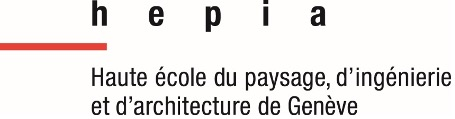
\includegraphics[width=5.86cm]{template/images/title/hepia_logo}};
\begin{spacing}{0.96}

	\begin{center}
		{\sf \fontsize{14pt}{16.8pt}\textsc{\textbf{\Orientation}}}\\*[1.5cm]
	\end{center}

	%% CONTENT STARTS HERE
	\noindent{\sf\textbf{Descriptif:}}
	La lumière Cherenkov est un phénomène physique similaire à un boom supersonique dans
	le domaine électromagnétique. Lorsque des particules chargées entrent dans notre atmosphère à
	la vitesse de la lumière, elles intéragissent avec les particules de celle-ci. 
	Ceci commence une réaction en chaîne produisant une pluie de rayonnements électromagnétiques
	et/ou de particules élémentaires telles que des protons par exemple.

	L'UNIGE travaille sur différents télescopes étudiant ce phénomène et souhaite améliorer
	la détection d'évènements intéressants physiquement pour réduire la quantité de données à stocker, transmettre et traiter.
	Pour cela, il est imaginé d'ajouter une étape de pré-traitement pour chaque pixel d'une caméra d'un télescope pour y filtrer
	le bruit des capteurs et effectuer une estimation calorifique du nombre de photons détectés.
	
	L'étape de pré-traitement utilisera le modèle de machine learning le plus capable à discerner 
	la ou les impulsions de photons à partir de la sortie analogique du capteur.

	\noindent{\sf\textbf{Travail demandé:}}
	Le travail demandé consiste à :
	\begin{itemize}
		\item Établir une série de tests et de métriques permettant de comparer différents modèles.
		\item Tester différents modèles de réseau de neurones (CNN/RNN/KAN).
		\item Intégrer l'étape de pré-traitement dans le pipeline du logiciel de classification de pluies Cherenkov : CTLearn.
		\item Exploration de l'utilisation du pré-traitement pour améliorer les performances de la stéréoscopie de CTLearn.
	\end{itemize}

	%% CONTENT ENDS HERE
	\vfill

	\begin{center}
		{\sf
			%%%%%%%%%%%%%%%%%%%%%%%%%%%%%%%%%%%%%%%%%%%%%%%%%%%%%%%%%%%%%%%%%%%%%%%%%%%%%%%%
			%%%%%%%%%%%%%%%%%%%%%%%%%% DO NOT MODIFY THE TABLE BELOW %%%%%%%%%%%%%%%%%%%%%%%
			%%%%%%%%%%%%%%%%%%%%%%%%%%%%%%%%%%%%%%%%%%%%%%%%%%%%%%%%%%%%%%%%%%%%%%%%%%%%%%%%
			\begin{tabular*}{16cm}{p{7.58cm} p{7.58cm}}
				\small Candidat-e:					&	\small Professeur-e(s) responsable(s):\\*[10pt]
				\small\textbf{\textsc{\Author}}		&	\small\textbf{\textsc{\Professor}}\\*[10pt]
				\footnotesize  Filière d’études : ISC	&	\footnotesize  \textbf{En collaboration avec:} UNIGE\\*[10pt]
				\footnotesize  {} & \footnotesize  Travail de bachelor soumis à une convention de stage en entreprise: \Convention\\*[20pt]
				\footnotesize  {} & \footnotesize  Travail soumis à un contrat de confidentialité: \Confidentiel\\*[10pt]
			\end{tabular*}\\*[0.5cm]
		}
	\end{center}
\end{spacing}
\end{document}
